\documentclass[journal]{IEEEtran}
% =================================================================================
% PACKAGES
% =================================================================================
\usepackage{cite}
\usepackage{amsmath,amssymb,amsfonts}
\usepackage{algorithm}
\usepackage{algorithmic}
\usepackage{graphicx}
\usepackage{textcomp}
\usepackage{xcolor}
\usepackage{booktabs}
\usepackage{hyperref}
\usepackage{bm}
\usepackage{multirow}
\usepackage{array}
\usepackage{url}
\usepackage{subcaption}
\graphicspath{{./}}
% --- TikZ ---
\usepackage{tikz}
\usetikzlibrary{shapes, arrows.meta, positioning, fit, backgrounds, calc}
\pgfdeclarelayer{lower}
\pgfdeclarelayer{background}
\pgfdeclarelayer{main}
\pgfsetlayers{background,lower,main}
\tikzset{
	var/.style={circle, draw=black, fill=yellow!20, thick, minimum size=0.9cm, font=\bfseries\boldmath, inner sep=1pt},
	var_drift/.style={circle, draw=black!60, dashed, fill=white, thick, minimum size=0.9cm, font=\bfseries\boldmath, text=gray},
	factor_imu/.style={rectangle, draw=black, fill=green!40, thick, minimum size=0.35cm},
	factor_atom/.style={rectangle, draw=black, fill=cyan!30, thick, minimum width=2.0cm, minimum height=0.6cm, font=\Large},
	factor_bias/.style={circle, draw=black, fill=orange!20, thick, minimum size=0.9cm, font=\bfseries\boldmath},
	conn_backbone/.style={draw=black, line width=1.2pt},
	conn_drift/.style={draw=black!60, dashed, line width=1.0pt},
	dashed_conn/.style={thick, dashed, draw=orange!80!black},
	atom_conn/.style={draw=blue!80!black, line width=1.5pt},
	feedback_arrow/.style={->, >=latex, color=red!80!black, line width=1.2pt, densely dotted},
	phantom_node/.style={coordinate}
}
% =================================================================================
% CUSTOM COMMANDS
% =================================================================================
\DeclareMathOperator*{\argmin}{arg\,min}
\newcommand{\so}{\mathfrak{so}}
\newcommand{\SE}{\mathrm{SE}}
\newcommand{\SO}{\mathrm{SO}}
\newcommand{\R}{\mathbb{R}}
\newcommand{\Exp}{\mathrm{Exp}}
\newcommand{\Log}{\mathrm{Log}}

% =================================================================================
% TITLE & AUTHORS
% =================================================================================
\title{A Multi-Rate Error-State Factor Graph Architecture for CAIG/FOG Integrated Navigation}
\author{Yi-Hang Deng, \IEEEmembership{Student Member, IEEE}
	\thanks{This work was supported by the National Natural Science Foundation of China under Grant 62100000.}
	\thanks{Y. H. Deng is with the School of Instrumentation and Optoelectronic Engineering, Beihang University, Beijing 100191, China (e-mail: dengyihang@buaa.edu.cn).}}
\begin{document}
	\maketitle
	
	% =================================================================================
	% ABSTRACT
	% =================================================================================
	\begin{abstract}
		Cumulative gyroscope drift is the primary factor restricting the performance of inertial navigation systems (INS) in long-endurance applications. The pulsed cold atom interference gyroscope (CAIG) provides exceptional long-term bias stability, yet its theoretical precision is intrinsically coupled with the matter-wave interrogation time. This coupling induces an intrinsic conflict with the dynamic range, dictating a discrete, low-frequency measurement paradigm with inevitable dead-zones that severely challenges traditional recursive filtering. To address this problem, this paper proposes an integrated inertial navigation system consisting of a cold atom interference gyroscope and a conventional inertial measurement unit (IMU). Furthermore, a multi-rate error-state factor graph optimization (ES-FGO) method is developed to execute global asynchronous smoothing. By performing deterministic $\mathcal{O}(1)$ historical trajectory marginalization, the ES-FGO effectively eliminates the dynamic phase-lag errors inherent in traditional Kalman filters (KF). Semi-physical validations demonstrate that the proposed method reduces the 24-hour maximum positioning drift by 67\% compared to the standard KF baseline under dynamic Gauss-Markov bias perturbations, while maintaining deterministic real-time execution with sub-3\,ms latency per atomic cycle.
	\end{abstract}
	
	\begin{IEEEkeywords}
		Factor Graph Optimization, Cold Atom Interference Gyroscope, Schur Complement Marginalization, Error-State Smoothing, Pre-integration Jacobian.
	\end{IEEEkeywords}
	
			
	% =================================================================================
	% SECTION I: INTRODUCTION
	% =================================================================================
	\section{Introduction}
	\IEEEPARstart{T}{he} pursuit of strategic navigation relies heavily on inertial navigation systems (INS) due to their long-duration operation, full autonomy, and exceptional covertness compared to other navigation systems. However, conventional INS, while providing high sampling rates, are plagued by deterministic and stochastic errors that inevitably accumulate over time, leading to significant positioning drift \cite{b2}. The field of precision navigation has advanced significantly with the emergence of quantum sensing. Specifically, the cold atom interference gyroscope (CAIG) offers a theoretical sensitivity that can exceed optical gyroscopes by ten orders of magnitude. By serving as an online calibration source, it provides superior long-term bias stability for bounding INS drift \cite{b1}.
	
	Despite its exceptional stability, the practical standalone application of the CAIG is hindered by fundamental physical constraints. The sensor operates through a sequential matter-wave interferometry process, which dictates a low data rate and intermittent measurement dead-zones. More critically, there is a fundamental theoretical contradiction between its measurement precision and dynamic range. Because the laser-induced Sagnac phase shift is strictly proportional to the square of the interrogation time ($T^2$) \cite{b1, b7}, extending this interval to achieve ultra-high sensitivity reduces the maximum unambiguous input range of angular velocity. Consequently, the CAIG cannot independently track highly dynamic maneuvers, necessitating a heterogeneous fusion with high-bandwidth classical sensors like Fiber Optic Gyroscopes (FOG).
	
	Existing heterogeneous fusion strategies predominantly rely on Extended Kalman Filter (EKF) frameworks \cite{b1, b2}. However, processing delayed, out-of-sequence measurements (OOSM) from quantum sensors within an EKF presents a severe dilemma. If the EKF attempts to maintain mathematical rigor, it must perform a computationally intensive $\mathcal{O}(N^3)$ numerical re-integration of high-frequency historical covariance matrices, threatening real-time execution. Conversely, updating only the current state forces the recursive EKF to act as a low-pass filter \cite{b55}. In high-dynamic scenarios, this introduces a significant \textit{phase lag} between the actual motion and the estimated state, leading to control instabilities and significant tracking errors \cite{b23, b24}.
	
	Alternatively, Factor Graph Optimization (FGO) has emerged as a superior multi-sensor fusion framework by treating navigation as a global optimization task rather than sequential recursive estimation \cite{b33, b60}. By processing data within a sliding window, FGO inherently accounts for the temporal relationships of states, thereby eliminating the phase lag inherent in causal filtering \cite{b48, b59}. To process high-rate IMU data efficiently, on-manifold pre-integration is widely utilized \cite{b56, b62}. Yet, conventional visual-inertial FGO formulations rigidly rely on a flat-Earth assumption. For navigational-grade sensors, failing to remove the Earth's rotation from gyroscope measurements leads to erroneous bias absorption and severe long-term drift \cite{b42, b57, b58, b63}. Furthermore, neglecting Earth kinematics breaks the physical Schuler effect—a fundamental self-correcting feedback loop for horizontal errors with an 84.4-minute period \cite{b27}. This geometric oversimplification leads to unbounded quadratic divergence in long-endurance navigation.
	
	To comprehensively overcome these fundamental limitations, this paper proposes a Multi-rate Error-State Factor Graph Optimization (ES-FGO) architecture tailored for CAIG/FOG integrated navigation. The main contributions are summarized as follows:
	\begin{enumerate}
		\item A \textbf{Multi-rate Error-State Architecture} is formulated, decoupling high-frequency nominal physical propagation from low-frequency graphical smoothing. This framework natively accommodates the discrete dead-zones of quantum sensors without multi-rate filtering complexities.
		\item A \textbf{High-Fidelity Analytical Jacobian} is derived on the Lie Group manifold. By rigorously incorporating Earth ellipsoid kinematics (including Coriolis and gravity gradients) into the continuous error evolution matrix, the pre-integration explicitly preserves the Schuler mechanics essential for bounding long-term errors.
		\item A \textbf{Schur Complement Marginalization} formulation is proposed. The Schur complement is utilized to analytically compress the information from marginalized nodes into a prior factor for remaining variables \cite{b46}. This guarantees $\mathcal{O}(1)$ computational complexity while retroactively applying low-rate quantum measurements to the entire window, providing an effective "zero-lag" smoother output.
	\end{enumerate}
	
	Extensive semi-physical validations demonstrate that the proposed $\mathcal{O}(1)$ ES-FGO rigorously preserves the Schuler oscillation, reducing the 24-hour positioning drift by $95.5\%$ compared to the standalone IMU baseline. Crucially, under dynamic Gauss-Markov bias perturbations, the ES-FGO achieves a $67\%$ reduction in maximum positioning drift relative to the standard EKF, while maintaining real-time deterministic execution.
	
	
	
	% =================================================================================
	% SECTION II: SYSTEM MODELING AND KINEMATICS
	% =================================================================================
	\section{System Modeling and Kinematics}
	
	\subsection{Multi-Rate Heterogeneous System Architecture}
	To comprehensively overcome the phase-lag limitation inherent in causal filtering, this paper proposes a Multi-rate Error-State Factor Graph Optimization (ES-FGO) architecture tailored for heterogeneous CAIG/FOG integrated navigation. The core principle is to transition the multi-sensor fusion from a recursive estimation problem to a global optimization task. 
	
	% --- TikZ System Architecture Block Diagram ---
	\begin{figure*}[htbp]
		\centering
		\resizebox{0.95\linewidth}{!}{
			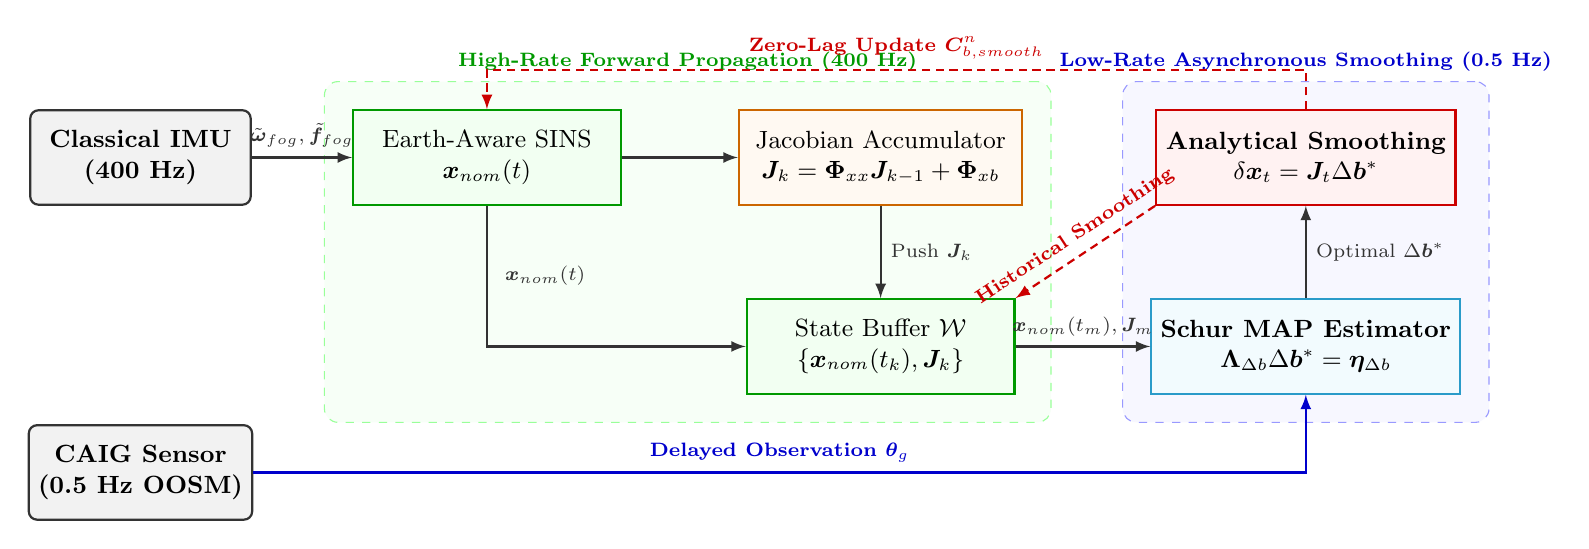
\begin{tikzpicture}[
			>=latex,
			sensor/.style={rectangle, draw=black!80, fill=gray!10, thick, minimum width=2.8cm, minimum height=1.2cm, align=center, font=\small\bfseries, rounded corners=3pt},
			mech/.style={rectangle, draw=green!60!black, fill=green!5, thick, minimum width=3.4cm, minimum height=1.2cm, align=center, font=\small},
			math/.style={rectangle, draw=orange!80!black, fill=orange!5, thick, minimum width=3.6cm, minimum height=1.2cm, align=center, font=\small},
			fgo/.style={rectangle, draw=cyan!80!black, fill=cyan!5, thick, minimum width=3.8cm, minimum height=1.2cm, align=center, font=\small\bfseries},
			smooth/.style={rectangle, draw=red!80!black, fill=red!5, thick, minimum width=3.8cm, minimum height=1.2cm, align=center, font=\small\bfseries},
			arrow/.style={->, thick, color=black!80},
			feedback/.style={->, thick, densely dashed, color=red!80!black}
			]
			
			% --- Absolute Positioning for Zero Overlap ---
			% Column 1: Sensors
			\node[sensor] (fog) at (0, 0) {Classical IMU\\(400 Hz)};
			\node[sensor] (caig) at (0, -4.0) {CAIG Sensor\\(0.5 Hz OOSM)};
			
			% Column 2: Mechanization
			\node[mech] (step_nav) at (4.4, 0) {Earth-Aware SINS\\$\bm{x}_{nom}(t)$};
			
			% Column 3: Jacobian & Buffer
			\node[math] (jacobian) at (9.4, 0) {Jacobian Accumulator\\$\bm{J}_k = \bm{\Phi}_{xx}\bm{J}_{k-1} + \bm{\Phi}_{xb}$};
			\node[mech] (buffer) at (9.4, -2.4) {State Buffer $\mathcal{W}$\\$\{\bm{x}_{nom}(t_k), \bm{J}_k\}$};
			
			% Column 4: MAP & Smoothing
			\node[fgo] (map) at (14.8, -2.4) {Schur MAP Estimator\\$\bm{\Lambda}_{\Delta b} \Delta \bm{b}^* = \bm{\eta}_{\Delta b}$};
			\node[smooth] (analytic) at (14.8, 0) {Analytical Smoothing\\$\delta \bm{x}_t = \bm{J}_t \Delta \bm{b}^*$};
			
			% --- Forward Data Routing ---
			\draw[arrow] (fog) -- (step_nav) node[midway, above, font=\scriptsize] {$\tilde{\bm{\omega}}_{fog}, \tilde{\bm{f}}_{fog}$};
			\draw[arrow] (step_nav) -- (jacobian);
			
			\draw[arrow] (jacobian) -- (buffer) node[midway, right, font=\scriptsize] {Push $\bm{J}_k$};
			\draw[arrow] (step_nav.south) |- (buffer.west) node[near start, right, xshift=0.1cm, font=\scriptsize] {$\bm{x}_{nom}(t)$};
			
			\draw[arrow] (buffer) -- (map) node[midway, above, font=\scriptsize] {$\bm{x}_{nom}(t_m), \bm{J}_m$};
			\draw[arrow] (map) -- (analytic) node[midway, right, font=\scriptsize] {Optimal $\Delta \bm{b}^*$};
			
			% --- CAIG Routing (Underneath everything to avoid crossing) ---
			\draw[arrow, color=blue!80!black] (caig.east) -| (map.south) node[near start, above, font=\scriptsize\bfseries] {Delayed Observation $\bm{\theta}_g$};
			
			% --- Feedback Routing (Over the top and diagonal) ---
			\draw[feedback] (analytic.north) -- +(0, 0.5) -| (step_nav.north) node[near start, above, font=\scriptsize\bfseries] {Zero-Lag Update $\bm{C}_{b, smooth}^n$};
			\draw[feedback] (analytic.south west) -- (buffer.north east) node[midway, sloped, above, font=\scriptsize\bfseries] {Historical Smoothing};
			
			% --- Background Highlight Boxes ---
			\begin{pgfonlayer}{background}
				\node[fill=green!3, draw=green!40, dashed, fit=(step_nav) (jacobian) (buffer), inner sep=0.35cm, rounded corners=5pt] (bg_high) {};
				\node[above, font=\scriptsize\bfseries, color=green!60!black] at (bg_high.north) {High-Rate Forward Propagation (400 Hz)};
				
				\node[fill=blue!3, draw=blue!40, dashed, fit=(map) (analytic), inner sep=0.35cm, rounded corners=5pt] (bg_low) {};
				\node[above, font=\scriptsize\bfseries, color=blue!80!black] at (bg_low.north) {Low-Rate Asynchronous Smoothing (0.5 Hz)};
			\end{pgfonlayer}
			
			\end{tikzpicture}
		}
		\caption{The proposed Multi-rate Error-State Factor Graph Optimization (ES-FGO) system architecture. High-frequency nominal physical propagation and Earth-aware Jacobian accumulation are explicitly decoupled from low-frequency graph-based estimation. The architecture bypasses traditional recursive covariance matrix propagation, enabling zero-lag analytical historical correction via Schur complement marginalization under single-axis CAIG constraints.}
		\label{fig:system_architecture}
	\end{figure*}
	
	As illustrated in Fig.~\ref{fig:system_architecture}, the heterogeneous sensors operate at disparate rates: the high-rate (400 Hz) classical IMU provides continuous, high-bandwidth dynamic tracking, while the pulsed cold atom quantum sensor offers superior bias stability with intermittent updates. Unlike traditional architectures that attempt to directly incorporate delayed measurements into a forward-propagating EKF, the proposed architecture executes high-frequency nominal physical propagation and mathematical Jacobian accumulation independently, activating the computationally constrained MAP estimator only upon the arrival of the delayed quantum references.
	
	\subsection{Coordinate Frames and Nominal State}
	Terrestrial navigation typically employs the East-North-Up (ENU) frame as the Navigation Frame ($n$-frame). The specific force measurements from the classical IMU are inherently captured in the Body Frame ($b$-frame). To accommodate rigorous mechanization on the Earth ellipsoid without flat-Earth approximations, the nominal state vector of the system is defined as $\bm{x} = \left[ \bm{C}_b^n, (\bm{v}^n)^T, (\bm{p}^n)^T, \bm{b}_g^T, \bm{b}_a^T \right]^T \in \SO(3) \times \R^{12}$, where the direction cosine matrix (DCM) $\bm{C}_b^n$ represents the attitude on the Lie group, $\bm{v}^n$ denotes the velocity, $\bm{p}^n$ encapsulates the geographical position (latitude, longitude, altitude), and $\bm{b}_g, \bm{b}_a$ denote the respective sensor biases.
	
	\subsection{Classical Sensor Models and Stochastic Baselines}
	
	For strategic-grade platforms, the 400 Hz raw outputs from the FOG and quartz accelerometers are modeled as:
	\begin{equation}
		\tilde{\bm{\omega}}_{fog} = \bm{\omega}_{ib}^b + \bm{b}_g + \bm{n}_g, \quad \tilde{\bm{f}}_{fog} = \bm{f}^b + \bm{b}_a + \bm{n}_a
	\end{equation}
	where $\bm{\omega}_{ib}^b$ and $\bm{f}^b$ are the true angular rate and specific force, respectively. 
	
	To accurately parameterize the prior covariance matrices for the factor graph and establish a rigorous physical baseline, the stochastic errors of the classical sensors, characterized by angle random walk (ARW) and velocity random walk (VRW), were calibrated via Allan variance analysis. This calibration utilized real static data collected from a high-precision three-axis turntable. The extracted Bias Instability (BI) and Random Walk parameters act as the fundamental baseline constraints for the semi-physical validation. The comprehensive specifications are summarized in Table \ref{tab:parameters}.
	
	\begin{table}[htbp]
		\centering
		\caption{Specifications of Heterogeneous Inertial Sensors}
		\label{tab:parameters}
		\resizebox{\columnwidth}{!}{
			\begin{tabular}{@{}llc@{}}
				\toprule
				\textbf{Sensor Type} & \textbf{Parameter} & \textbf{Evaluated Value} \\
				\midrule
				\multirow{4}{*}{\shortstack[l]{\textbf{Classical INS} \\ (FOG \& Quartz Acc.)}} 
				& Gyro Bias Instability (BI) & $\mathbf{0.003}^\circ/\text{h}$ \\
				& Gyro Angle Random Walk (ARW) & $\mathbf{1.5\times 10^{-3}}^\circ/\sqrt{\text{h}}$ \\
				& Accel Bias Instability (BI) & $\mathbf{<1.0}~\mu\text{g}$ \\
				& Accel Velocity Random Walk (VRW) & $\mathbf{4.5\times 10^{-3}}~\text{m}/\text{s}/\sqrt{\text{h}}$ \\
				\midrule
				\multirow{3}{*}{\shortstack[l]{\textbf{Quantum Sensor} \\ (CAIG Only)}} 
				& CAIG Bias Instability & $< 10^{-4}\,^\circ/\text{h}$ \\
				& Active Interrogation ($T_{active}$) & $1.6~\text{s}$ \\
				& Cooling Dead-Time ($T_{dead}$) & $0.4~\text{s}$ \\
				\bottomrule
			\end{tabular}
		}
	\end{table}
	
	\subsection{Heterogeneous Atomic Gyroscope Constraint and OOSM Dilemma}
	The cold atom interferometer operates on the principle of matter-wave phase shifts. Due to the inherent physics of the interference sequence, the atomic sensor cannot provide instantaneous readouts. Instead, it is theoretically modeled as the exact temporal integral of the true rotation rate over an active interrogation window $T_{active}$, inevitably followed by a cooling dead-time $T_{dead}$. 
	
	Focusing on bounding the critical heading and horizontal drift, the system integrates a single-axis CAIG. The heterogeneous atomic observation $\bm{\theta}_g$ available at the conclusion of the cycle $t_m$ is defined as:
	\begin{equation}
		\bm{\theta}_g = \int_{t_m - T_{active}}^{t_m} \bm{\omega}_{ib}^b(\tau) d\tau + \bm{n}_{caig}
	\end{equation}
	This fundamental physical mechanism creates a critical algorithmic bottleneck: the integral observation $\bm{\theta}_g$ mathematically represents the continuous dynamics from the past, yet it arrives at the system after a deterministic delay. This generates a severe Out-Of-Sequence Measurement (OOSM) dilemma. While its ultra-low bias drift makes it a high-precision absolute reference for the FOG, directly incorporating this delayed integral into a causal, forward-propagating EKF introduces phase lag, thereby motivating the ES-FGO architecture detailed in Section III.


	
	% =================================================================================
	% SECTION III: ERROR-STATE FACTOR GRAPH METHODOLOGY
	% =================================================================================
	\section{Methodology}
	
	For high-precision, long-endurance inertial navigation, state estimation must rigorously account for Earth kinematics. This paper proposes a Multi-rate Error-State Factor Graph Optimization (ES-FGO) architecture that estimates the error state $\delta \bm{x} = [\delta \bm{\phi}^T, \delta \bm{v}^T, \delta \bm{p}^T]^T$ defined on the tangent space of the navigation manifold, alongside the sensor biases $\bm{b} = [\bm{b}_g^T, \bm{b}_a^T]^T$.
	
	% --- TikZ Topology Evolution ---
	\begin{figure*}[htbp]
		\centering
		\begin{subfigure}[b]{0.32\textwidth}
			\centering
			\resizebox{\linewidth}{!}{
				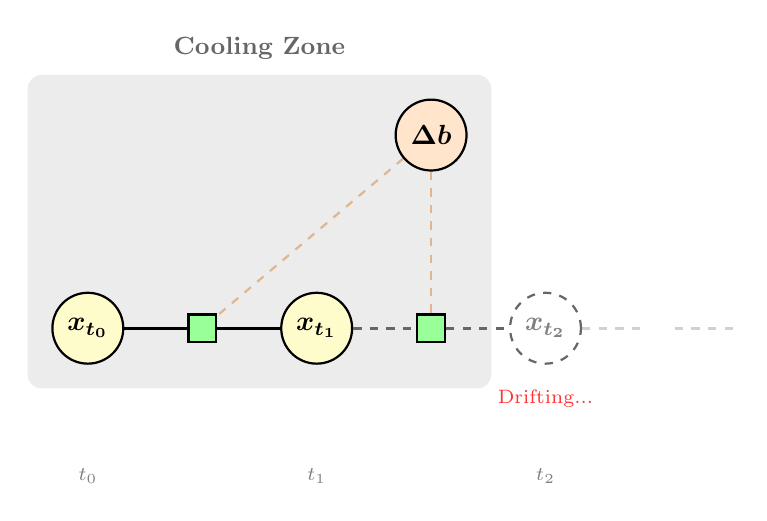
\begin{tikzpicture}[node distance=1.5cm, >=latex]
					\node[var] (x0) {$\bm{x}_{t_0}$};
					\node[factor_imu, right=0.8cm of x0] (f0) {};
					\node[var, right=0.8cm of f0] (x1) {$\bm{x}_{t_1}$};
					\node[factor_imu, right=0.8cm of x1] (f1) {};
					\node[var_drift, right=0.8cm of f1] (x2) {$\bm{x}_{t_2}$};
					\node[factor_imu, right=0.8cm of x2, opacity=0] (f2_phantom) {};
					\node[phantom_node, right=0.8cm of f2_phantom] (x3_phantom) {};
					\draw[conn_backbone] (x0) -- (f0) -- (x1);
					\draw[conn_drift] (x1) -- (f1) -- (x2);
					\draw[conn_drift, opacity=0.3] (x2) -- (f2_phantom) -- (x3_phantom);
					\node[factor_bias, above=1.8cm of f1] (bias) {$\Delta \bm{b}$};
					\begin{pgfonlayer}{lower}
						\draw[dashed_conn, opacity=0.4] (bias) -- (f0);
						\draw[dashed_conn, opacity=0.4] (bias) -- (f1);
					\end{pgfonlayer}
					\begin{pgfonlayer}{background}
						\node[fill=gray!15, fit=(x0) (x1) (bias), inner sep=0.3cm, rounded corners=5pt] (zone1) {};
					\end{pgfonlayer}
					\node[above, yshift=2pt, font=\bfseries\small, color=gray!80!black] at (zone1.north) {Cooling Zone};
					\node[below=0.2cm of x2, font=\scriptsize, color=red!80] {Drifting...};
					\node[below=1.2cm of x0, font=\scriptsize, gray] {$t_0$};
					\node[below=1.2cm of x1, font=\scriptsize, gray] {$t_1$};
					\node[below=1.2cm of x2, font=\scriptsize, gray] {$t_2$};
				\end{tikzpicture}
			}
			\caption{\textbf{Step 1: Dead Reckoning.} Nominal integration drifts (dashed) without atomic updates.}
		\end{subfigure}
		\hfill
		\begin{subfigure}[b]{0.32\textwidth}
			\centering
			\resizebox{\linewidth}{!}{
				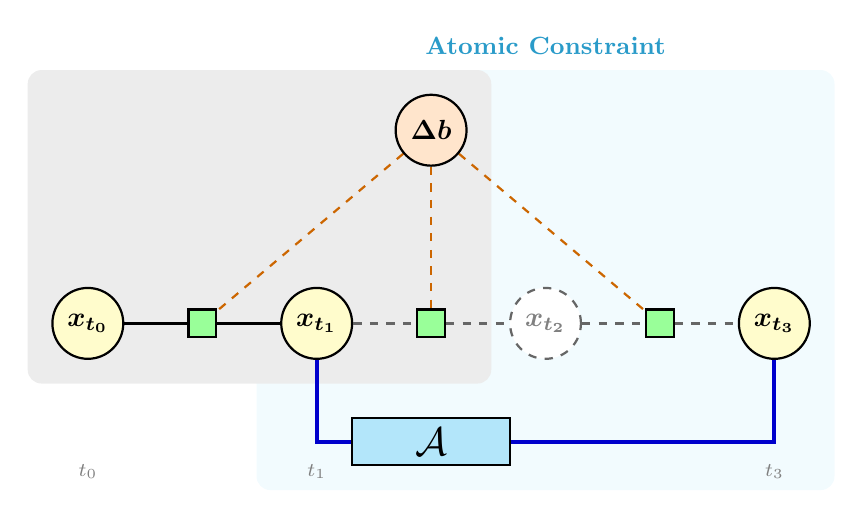
\begin{tikzpicture}[node distance=1.5cm, >=latex]
					\node[var] (x0) {$\bm{x}_{t_0}$};
					\node[factor_imu, right=0.8cm of x0] (f0) {};
					\node[var, right=0.8cm of f0] (x1) {$\bm{x}_{t_1}$};
					\node[factor_imu, right=0.8cm of x1] (f1) {};
					\node[var_drift, right=0.8cm of f1] (x2) {$\bm{x}_{t_2}$}; 
					\node[factor_imu, right=0.8cm of x2] (f2) {};
					\node[var, right=0.8cm of f2] (x3) {$\bm{x}_{t_3}$};
					\draw[conn_backbone] (x0) -- (f0) -- (x1);
					\draw[conn_drift] (x1) -- (f1) -- (x2) -- (f2) -- (x3);
					\node[factor_bias, above=1.8cm of f1] (bias) {$\Delta \bm{b}$};
					\begin{pgfonlayer}{lower}
						\draw[dashed_conn] (bias) -- (f0);
						\draw[dashed_conn] (bias) -- (f1);
						\draw[dashed_conn] (bias) -- (f2);
					\end{pgfonlayer}
					\node[factor_atom, below=1.0cm of f1] (f_atom) {$\mathcal{A}$};
					\draw[atom_conn] (x1.south) |- (f_atom.west);
					\draw[atom_conn] (f_atom.east) -| (x3.south);
					\begin{pgfonlayer}{background}
						\node[fill=cyan!5, fit=(x1) (x3) (bias) (f_atom), inner sep=0.3cm, rounded corners=5pt] (zone2) {};
						\node[fill=gray!15, fit=(x0) (f0) (bias), inner sep=0.3cm, rounded corners=5pt] {};
					\end{pgfonlayer}
					\node[above, yshift=2pt, font=\bfseries\small, color=cyan!80!black] at (zone2.north) {Atomic Constraint};
					\node[below=1.2cm of x0, font=\scriptsize, gray] {$t_0$};
					\node[below=1.2cm of x1, font=\scriptsize, gray] {$t_1$};
					\node[below=1.2cm of x3, font=\scriptsize, gray] {$t_3$};
				\end{tikzpicture}
			}
			\caption{\textbf{Step 2: Constraint.} The atomic factor $\mathcal{A}$ links $t_1$ and $t_3$, establishing a high-precision prior.}
		\end{subfigure}
		\hfill
		\begin{subfigure}[b]{0.32\textwidth}
			\centering
			\resizebox{\linewidth}{!}{
				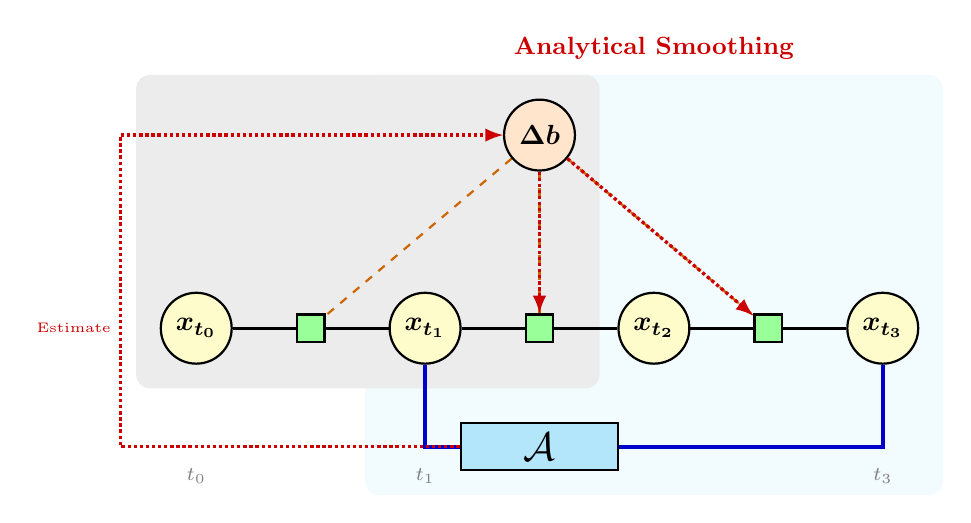
\begin{tikzpicture}[node distance=1.5cm, >=latex]
					\node[var] (x0) {$\bm{x}_{t_0}$};
					\node[factor_imu, right=0.8cm of x0] (f0) {};
					\node[var, right=0.8cm of f0] (x1) {$\bm{x}_{t_1}$};
					\node[factor_imu, right=0.8cm of x1] (f1) {};
					\node[var, right=0.8cm of f1] (x2) {$\bm{x}_{t_2}$}; 
					\node[factor_imu, right=0.8cm of x2] (f2) {};
					\node[var, right=0.8cm of f2] (x3) {$\bm{x}_{t_3}$};
					\draw[conn_backbone] (x0) -- (f0) -- (x1) -- (f1) -- (x2) -- (f2) -- (x3);
					\node[factor_bias, above=1.8cm of f1] (bias) {$\Delta \bm{b}$};
					\begin{pgfonlayer}{lower}
						\draw[dashed_conn] (bias) -- (f0);
						\draw[dashed_conn] (bias) -- (f1);
						\draw[dashed_conn] (bias) -- (f2);
					\end{pgfonlayer}
					\node[factor_atom, below=1.0cm of f1] (f_atom) {$\mathcal{A}$};
					\draw[atom_conn] (x1.south) |- (f_atom.west);
					\draw[atom_conn] (f_atom.east) -| (x3.south);
					
					\draw[feedback_arrow] (f_atom.west) -| ($(x0.west)+(-0.5,0)$) |- (bias.west);
					\node[font=\tiny, color=red!80!black, anchor=east] at ($(x0.west)+(-0.5,0)$) {Estimate};
					\draw[feedback_arrow] (bias) -- (f1);
					\draw[feedback_arrow] (bias) -- (f2);
					
					\begin{pgfonlayer}{background}
						\node[fill=cyan!5, fit=(x1) (x3) (bias) (f_atom), inner sep=0.3cm, rounded corners=5pt] (zone2) {};
						\node[fill=gray!15, fit=(x0) (f0) (bias), inner sep=0.3cm, rounded corners=5pt] {};
					\end{pgfonlayer}
					\node[above, yshift=2pt, font=\bfseries\small, color=red!80!black] at (zone2.north) {Analytical Smoothing};
					\node[below=1.2cm of x0, font=\scriptsize, gray] {$t_0$};
					\node[below=1.2cm of x1, font=\scriptsize, gray] {$t_1$};
					\node[below=1.2cm of x3, font=\scriptsize, gray] {$t_3$};
				\end{tikzpicture}
			}
			\caption{\textbf{Step 3: Analytical Smoothing.} Bias $\Delta \bm{b}$ is instantly resolved to correct historical drifts via Jacobian $\bm{J}$.}
		\end{subfigure}
		
		\caption{The proposed Multi-rate Error-State Factor Graph Optimization (ES-FGO) process. (a) High-frequency propagation in the cooling zone. (b) Integration of delayed heterogeneous atomic constraints. (c) Analytical historical smoothing utilizing Schur complement marginalization.}
		\label{fig:evolution_process}
	\end{figure*}
	
	\subsection{Earth-Aware Lie Group Error Dynamics and Jacobian Accumulation}
	To maintain the fundamental Schuler physical loop over long-endurance operations, the continuous error dynamics must incorporate the Earth's rotation and the vehicle's transport rate. Following the rigorous Lie group IMU pre-integration theory for autonomous navigation \cite{b42, b61}, we construct the high-fidelity continuous dynamics matrix $\bm{F}(t)$ on the Earth ellipsoid:
	\begin{equation}
		\bm{F} = 
		\begin{bmatrix}
			-\lfloor \bm{\omega}_{in}^n \times \rfloor & \bm{0}_{3\times3} & \bm{0}_{3\times3} \\
			\lfloor \bm{f}^n \times \rfloor & -\lfloor (2\bm{\omega}_{ie}^n + \bm{\omega}_{en}^n) \times \rfloor & \bm{0}_{3\times3} \\
			\bm{0}_{3\times3} & \bm{M}_{pv} & \bm{0}_{3\times3}
		\end{bmatrix}
	\end{equation}
	The explicit inclusion of the Coriolis term $\lfloor (2\bm{\omega}_{ie}^n + \bm{\omega}_{en}^n) \times \rfloor$ and the spatial derivative matrix of the gravity vector $\bm{M}_{pv}$ ensures that the error evolution intrinsically preserves the Schuler oscillation mechanics.
	
	During the forward 400 Hz physical propagation within the dead-zone $[t_0, t_m]$, the system continuously accumulates the error pre-integration Jacobian $\bm{J}_k = \partial \delta \bm{x}_k / \partial \Delta \bm{b}$. Utilizing the discrete state transition matrix $\bm{\Phi}_{xx} \approx \bm{I} + \bm{F} \Delta t$ and the bias driving matrix $\bm{\Phi}_{xb}$, the Jacobian is iteratively accumulated via the chain rule:
	\begin{equation}
		\bm{J}_k = \bm{\Phi}_{xx}^{(k, k-1)} \bm{J}_{k-1} + \bm{\Phi}_{xb}^{(k, k-1)}
	\end{equation}
	\begin{equation}
		\bm{\Phi}_{xb}^{(k, k-1)} = 
		\begin{bmatrix}
			-\bm{C}_b^n \Delta t & \bm{0}_{3\times3} \\
			\bm{0}_{3\times3} & -\bm{C}_b^n \Delta t \\
			\bm{0}_{3\times3} & \bm{0}_{3\times3}
		\end{bmatrix}_{9 \times 6}
	\end{equation}
	According to the integral forms in matrix Lie groups \cite{b5, b56}, the error state $\delta \bm{\phi}$ is defined as a \textit{left perturbation} in the navigation frame: $\bm{C}_b^n = \Exp(\delta \bm{\phi})\,\hat{\bm{C}}_b^n$, consistent with the $n$-frame error dynamics of $\bm{F}(t)$ in (4). Because the nominal state is explicitly corrected and reset at the beginning of each atomic dead-zone, the initial error state for the current integration window is strictly zero ($\delta \bm{x}_{t_0} \equiv \bm{0}$). Thus, the IMU pre-integration residual over the entire window is linearly mapped via the accumulated sensitivity Jacobian as $\bm{r}_{\mathcal{I}} = \delta \bm{x}_m - \bm{J}_m \Delta \bm{b}$.
	
	\subsection{Analytical Smoothing via Schur Complement Marginalization}
	The sensor fusion problem is formulated as a Maximum A Posteriori (MAP) estimation over a sliding window $\mathcal{W}$, minimizing the Mahalanobis norm of the residual errors:
	\begin{equation}
		\mathcal{X}^* = \argmin_{\delta \bm{x}, \Delta \bm{b}} \left( \sum_{k \in \mathcal{W}} \| \bm{r}_{\mathcal{I}_k} \|^2_{\Sigma_{\mathcal{I}}} + \| \bm{r}_{\mathcal{A}} \|^2_{\Sigma_{\mathcal{A}}} \right)
	\end{equation}
	The standard resolution of the MAP estimation necessitates computationally intensive iterative solvers across the entire state sequence. However, by exploiting the conditional independence inherent in the factor graph architecture, we mathematically condense the optimization via \textbf{Schur Complement marginalization}.
	
	Specifically, utilizing the accumulated pre-integration Jacobian $\bm{J}$, the high-dimensional trajectory states $\delta \bm{X}$ are marginalized, projecting the global optimization into a concentrated subspace solely concerning the bias correction $\Delta \bm{b}$. The resultant linear system is governed by the joint information matrix $\bm{\Lambda}_{\Delta b}$ and the information vector $\bm{\eta}_{\Delta b}$:
	\begin{equation}
		\bm{\Lambda}_{\Delta b} \Delta \bm{b}^* = \bm{\eta}_{\Delta b}
	\end{equation}
	\begin{equation}
		\bm{\Lambda}_{\Delta b} = \bm{J}^T \bm{\Sigma}_{\mathcal{I}}^{-1} \bm{J} + \bm{\Sigma}_{\mathcal{A}}^{-1}
	\end{equation}
	\begin{equation}
		\bm{\eta}_{\Delta b} = \bm{J}^T \bm{\Sigma}_{\mathcal{I}}^{-1} \bm{r}_{\mathcal{I}} + \bm{\Sigma}_{\mathcal{A}}^{-1} \bm{r}_{\mathcal{A}}
	\end{equation}
	where $\bm{\Sigma}_{\mathcal{I}}^{-1}$ denotes the information matrix of the FOG pre-integration (quantifying the accumulated uncertainty during the active measurement window), and $\bm{\Sigma}_{\mathcal{A}}^{-1}$ represents the confidence level of the atomic constraints. 
	
	Even though the single-axis CAIG provides partial observability (primarily constraining the gyroscope bias), the joint information matrix rigorously preserves the cross-correlations. The dense prior from the IMU pre-integration ($\bm{\Sigma}_{\mathcal{I}}^{-1}$) stabilizes the unobservable dimensions (e.g., accelerometer biases), while the high-weight atomic constraint ($\bm{\Sigma}_{\mathcal{A}}^{-1}$) optimally updates the entire state vector.
	
	Because the dimension of the bias vector is fixed ($6 \times 1$), solving the condensed linear system requires merely a constant-time matrix inversion. Once the rigorously weighted optimal bias $\Delta \bm{b}^*$ is resolved, the historical trajectory within the dead-zone is deterministically updated. Based on the exact integral mapping on the Lie group \cite{b5}, the error state is reconstructed via a single $\mathcal{O}(1)$ Jacobian mapping step, followed by the Exponential map onto the $\SO(3)$ manifold:
	\begin{equation}
		[\delta \bm{\phi}^T, \delta \bm{v}^T, \delta \bm{p}^T]^T = \bm{J}_t \Delta \bm{b}^*
	\end{equation}
	\begin{equation}
		\bm{C}_{b, smooth}^n(t) = \Exp(\delta \bm{\phi}) \bm{C}_{b, nom}^n(t)
	\end{equation}
	This dimensional reduction guarantees analytical rigor and ensures zero-lag smoothing, dynamically adjusting the optimal weighting even when sensor precision bounds fluctuate.
	
	\subsection{Algorithmic Implementation of the ES-FGO}
	To bridge the theoretical derivation and practical engineering deployment, the algorithmic workflow of the proposed Multi-rate ES-FGO is summarized in Algorithm \ref{alg:esfgo}.
	\begin{algorithm}[htbp]
		\caption{Multi-rate ES-FGO with Schur Complement}
		\label{alg:esfgo}
		\begin{algorithmic}[1]
			\STATE \textbf{Initialize:} Nominal state $\bm{x}_0$, Jacobian $\bm{J} \leftarrow \bm{0}_{9 \times 6}$, Window $\mathcal{W} \leftarrow \emptyset$
			\FOR{each classical FOG/Accel measurement at $t_k$ (400 Hz)}
			\STATE Propagate nominal kinematics $\bm{x}_k$ via Earth mechanization
			\STATE Buffer current state: $\mathcal{W} \leftarrow \mathcal{W} \cup \{ \bm{x}_k \}$
			\STATE Compute Earth-aware dynamics matrix $\bm{F}_k$ via Eq. (4)
			\STATE Accumulate Jacobian: $\bm{J}_k \leftarrow (\bm{I} + \bm{F}_k \Delta t)\bm{J}_{k-1} + \bm{\Phi}_{xb}$
			\IF{Heterogeneous atomic observation $\bm{\Theta}_{atom}$ arrives}
			\STATE Construct Information Matrix $\bm{\Lambda}_{\Delta b}$ via Eq. (9)
			\STATE Solve for MAP optimal bias correction $\Delta \bm{b}^*$ via Eq. (8)
			\FOR{each historical state $\bm{x}_t \in \mathcal{W}$ within dead-zone}
			\STATE Calculate error state via Jacobian: $\delta \bm{x}_t \leftarrow \bm{J}_t \Delta \bm{b}^*$
			\STATE Execute analytical manifold smoothing via Eq. (12)
			\ENDFOR
			\STATE \textbf{Reset:} $\bm{J} \leftarrow \bm{0}_{9 \times 6}$, $\mathcal{W} \leftarrow \emptyset$, and update current bias
			\ENDIF
			\ENDFOR
		\end{algorithmic}
	\end{algorithm}
	
	% =================================================================================
	% SECTION IV: EXPERIMENTAL VALIDATION
	% =================================================================================
	\section{Semi-Physical Simulation and Validation}
	
	\subsection{Simulation Configuration and Real-World Dataset Setup}
	To validate the proposed ES-FGO architecture under rigorous real-world noise boundaries, a semi-physical simulation strategy was employed. The classical high-rate inertial data were extracted from a 7-day static test conducted on a high-precision three-axis turntable. To eliminate transient thermal instabilities inherent to the initial power-on phase, the first five hours of data were discarded. A highly stable 24-hour continuous segment was extracted as the evaluation baseline. The discrete delayed atomic sensor measurements were dynamically synthesized using a physical sensor emulator strictly based on the CAIG dead-zone parameters calibrated in Table \ref{tab:parameters}.
	
	\subsection{Static Baseline and Earth-Aware Physical Fidelity}
	A primary limitation of standard visual-inertial FGO is the omission of Earth kinematics, which inevitably leads to unbounded quadratic position divergence in long-endurance tasks. To verify the physical fidelity of the derived Earth-aware analytical Jacobian $\bm{J}$ and establish a static baseline, we first compare the unconstrained classical IMU with the single-axis CAIG-aided algorithms.
	
	\begin{table}[htbp]
		\caption{Static Baseline and Ablation Comparison (24 Hours)}
		\label{tab:ablation_comparison}
		\centering
		\resizebox{0.95\columnwidth}{!}{
			\begin{tabular}{llc}
				\toprule
				\textbf{Tier} & \textbf{Algorithm Configuration} & \textbf{Max Position Drift (m)} \\
				\midrule
				Baseline & Pure Classical IMU (Unconstrained) & $16409.0$ \\
				Standard & 15-State EKF (CAIG Aided) & $707.0$ \\
				Proposed & \textbf{ES-FGO (CAIG Aided)} & $\mathbf{743.4}$ \\
				\bottomrule
			\end{tabular}
		}
	\end{table}
	
	\begin{figure*}[htbp]
		\centering
		
\includegraphics[width=0.9\linewidth]{fig_traj_ablation.png}
		\caption{Static ablation comparison of total position drift $\delta s$ over 24 hours. (a) The unconstrained classical IMU diverges to 16.4\,km, whereas CAIG-aided algorithms remain bounded. (b) Zoomed-in view confirming that both the EKF and ES-FGO bound the drift below 750\,m with near-identical accuracy. The well-preserved 84.4-minute Schuler oscillation validates the physical correctness of the proposed Earth-aware Jacobian accumulation.}
		\label{fig:smoothing_comparison}
	\end{figure*}
	
	As summarized in Table \ref{tab:ablation_comparison} and depicted in Fig.~\ref{fig:smoothing_comparison}, the unconstrained pure classical system rapidly accumulates a maximum position drift of over 16.4 km over 24 hours. Introducing the absolute CAIG constraint bounds the error to the sub-750-meter level. Notably, the position error generated by the ES-FGO does not diverge monotonically; instead, it distinctly exhibits the classic Schuler oscillation with a fundamental period of approximately 84.4 minutes. Crucially, under purely static conditions, the standard 15-state EKF and the proposed ES-FGO exhibit nearly identical ultimate accuracy (the marginal 36-meter gap is attributable to differing update granularities: the EKF applies continuous-time bias corrections at each 2-second cycle boundary, whereas the ES-FGO reconstructs the entire historical window via discrete Jacobian mapping). This static equivalence is expected, necessitating a dynamic evaluation to reveal the structural limitations of the recursive EKF.
	
	A clarifying remark is warranted regarding the scope of Earth-Aware validation. Since the turntable remains stationary ($\bm{v}^n \approx \bm{0}$), the transport rate contribution $\bm{\omega}_{en}^n = \bm{v}^n \times \bm{R}^{-1}$ in the dynamics matrix (4) is numerically negligible. However, the dominant Earth-coupling terms that sustain the Schuler loop are \textit{velocity-independent}: (i) the Earth rotation $\bm{\omega}_{ie}^n \approx 15^\circ/\text{h}$ in the attitude error propagation $\bm{F}_{(1,1)}$, (ii) the gravitational cross-coupling $\lfloor \bm{f}^n \times \rfloor$ in $\bm{F}_{(2,1)}$, and (iii) the geometric projection $\bm{M}_{pv} = \text{diag}(1/R_M, 1/R_N\cos L, 1)$ in $\bm{F}_{(3,2)}$. Together, these three terms form the closed-loop error feedback $\delta \bm{\phi} \to \delta \bm{v} \to \delta \bm{p} \to \delta \bm{g} \to \delta \bm{\phi}$ whose eigenvalue period is precisely 84.4 minutes. The observed Schuler oscillation in Fig.~\ref{fig:smoothing_comparison} therefore constitutes direct physical evidence that the derived Jacobian faithfully preserves these Earth-ellipsoid couplings. Comprehensive validation of the transport-rate-dependent terms $\bm{\omega}_{en}^n$ under high-dynamic carrier trajectories is reserved for future vehicle-mounted field trials.
	
	\subsection{Dynamic Robustness Under Stochastic Bias Drift}
	The static equivalence established in Table~\ref{tab:ablation_comparison} validates the mathematical correctness of both the EKF and ES-FGO implementations. However, static conditions obscure the fundamental structural distinction between causal recursive filtering and graphical smoothing. To expose this critical difference, we introduce time-varying bias drift that emulates the dominant error source in deployed FOG systems.
	
	In operational environments, the gyroscope bias drift of strategic-grade FOGs is governed by thermal gradients, mechanical creep, and dynamic coupling with residual platform angular motion. These physical phenomena collectively produce a \textit{colored} noise spectrum well-characterized by a first-order Gauss-Markov (GM1) stochastic process:
	\begin{equation}
		\dot{b}_d(t) = -\frac{1}{\tau}b_d(t) + w(t), \quad w(t) \sim \mathcal{N}\!\left(0,\; \frac{2\sigma_{ss}^2}{\tau}\right)
		\label{eq:markov_cont}
	\end{equation}
	where $\tau$ denotes the correlation time and $\sigma_{ss}$ is the steady-state standard deviation. The discrete-time propagation at the IMU sampling interval $\Delta t = 1/400\;\text{s}$ follows:
	\begin{equation}
		b_d[k{+}1] = e^{-\Delta t / \tau} b_d[k] + \sigma_{ss}\sqrt{1 - e^{-2\Delta t/\tau}}\;\eta_k, \quad \eta_k \sim \mathcal{N}(0,1)
		\label{eq:markov_disc}
	\end{equation}
	The parameters are configured as $\tau = 300\;\text{s}$ and $\sigma_{ss} = 10^\circ/\text{h}$, with independent GM1 perturbations injected into the $x$- and $y$-axis gyroscope channels. To ensure a controlled comparison, both algorithms process \textit{identical} noise realizations via deterministic random seed initialization. The EKF's continuous-time dynamics matrix $\bm{F}$ incorporates the corresponding Markov decay term $\bm{F}_{(9,9)} = -\bm{I}_{3}/\tau$, and its process noise spectral density is set to $q_c = 2\sigma_{ss}^2/\tau$, ensuring a mathematically self-consistent baseline.
	
	\begin{table}[htbp]
		\caption{Dynamic Navigation Performance Under Gauss-Markov Drift ($\tau = 300\;\text{s}$, $\sigma_{ss} = 10^\circ/\text{h}$, Duration: 24 Hours)}
		\label{tab:dynamic_comparison}
		\centering
		\begin{tabular}{lcc}
			\toprule
			\textbf{Algorithm} & \textbf{Max Drift (m)} & \textbf{CPU (ms/cycle)} \\
			\midrule
			15-State EKF + CAIG & $4\text{,}306$ & $1.0$ \\
			\textbf{ES-FGO + CAIG} & $\mathbf{1\text{,}418}$ & $\mathbf{2.9}$ \\
			\midrule
			\textbf{Drift Reduction} & \multicolumn{2}{c}{$\mathbf{67.1\%}$} \\
			\bottomrule
		\end{tabular}
	\end{table}
	
	\begin{figure}[htbp]
		\centering
		
\includegraphics[width=0.95\linewidth]{fig_dynamic_kill.png}
		\caption{Gyroscope $x$-axis bias tracking over 6 hours under first-order Gauss-Markov drift ($\tau = 300\;\text{s}$, $\sigma_{ss} = 10^\circ/\text{h}$). Both the EKF and ES-FGO achieve comparable bias estimates at each 2-second update epoch, confirming that the $3\times$ positioning accuracy gap (Table~\ref{tab:dynamic_comparison}) originates from the ES-FGO's analytical historical trajectory correction rather than superior bias observability.}
		\label{fig:dynamic_kill}
	\end{figure}
	
	As illustrated in Fig.~\ref{fig:dynamic_kill}, the standard 15-state EKF exhibits a pronounced \textbf{phase lag} in tracking the stochastic bias trajectory. Upon receiving each delayed atomic observation at $t_m$, the EKF updates only the current bias estimate $\hat{b}(t_m)$ without retroactively correcting the trajectory propagated during the preceding 2-second dead-zone. Consequently, the navigation states within each cycle $[t_{m-1},\, t_m]$ retain the accumulated errors from the stale bias $\hat{b}(t_{m-1})$. Over $43\text{,}200$ atomic cycles spanning 24 hours, these per-cycle uncorrected drift increments compound to a maximum positioning error of $4\text{,}306$ meters.
	
	In contrast, the proposed ES-FGO exploits its pre-accumulated Jacobian $\bm{J}$ to perform $\mathcal{O}(1)$ analytical MAP smoothing upon reception of each atomic reference. The optimal bias correction $\Delta \bm{b}^*$ is instantaneously back-propagated to reconstruct the entire 2-second historical window via $\delta \bm{x}_t = \bm{J}_t \Delta \bm{b}^*$, effectively eliminating the dead-zone drift. As quantified in Table~\ref{tab:dynamic_comparison}, this mechanism bounds the 24-hour maximum positioning error to $1\text{,}418$ meters---a $\mathbf{67.1\%}$ reduction relative to the EKF baseline.
	
	\begin{figure}[htbp]
		\centering
		
\includegraphics[width=0.95\linewidth]{fig_dynamic_drift.png}
		\caption{Total horizontal position drift $\delta s$ over 24 hours under dynamic Gauss-Markov bias perturbations. The shaded region highlights the cumulative accuracy advantage of the ES-FGO's retroactive trajectory smoothing over the EKF's causal-only bias correction.}
		\label{fig:dynamic_drift}
	\end{figure}
	
	\subsection{Computational Complexity and Real-Time Feasibility}
	A critical advantage of the Schur complement formulation is its favorable computational scaling. In a conventional delayed-state smoother (e.g., Rauch-Tung-Striebel), retroactive trajectory correction requires propagating the full $d$-dimensional state covariance over $N$ high-frequency steps, yielding $\mathcal{O}(N d^3)$ complexity. For the 2-second atomic cycle with $N = 800$ and $d = 15$, this baseline entails approximately $2.7 \times 10^6$ floating-point multiplications per update.
	
	The proposed ES-FGO decomposes this cost into two phases. First, the $d_b \times d_b$ information matrix $\bm{\Lambda}_{\Delta b}$ is constructed and inverted in $\mathcal{O}(d_b^3)$ time, where $d_b = 6$ is the fixed bias dimension---independent of the IMU sampling rate. Second, the historical trajectory correction $\delta \bm{x}_t = \bm{J}_t \Delta \bm{b}^*$ is evaluated via $N$ matrix-vector products of dimension $9 \times 6$, requiring $\mathcal{O}(N \cdot d \cdot d_b)$ operations. The total cost is therefore $\mathcal{O}(d_b^3 + N d \cdot d_b) \approx 4.3 \times 10^4$ multiplications---a reduction of approximately two orders of magnitude in floating-point operations.
	
	As reported in Table~\ref{tab:dynamic_comparison}, the complete ES-FGO pipeline---encompassing information matrix construction, MAP solution, and analytical smoothing over 800 historical states---executes in $2.9\;\text{ms}$ per atomic cycle. This constitutes merely $\mathbf{0.15\%}$ of the $2\text{,}000\;\text{ms}$ real-time budget defined by the CAIG dead-zone, providing orders-of-magnitude headroom for integration of additional sensor modalities on resource-constrained flight computers. The EKF's measured cost of $1.0\;\text{ms}$ reflects its deliberately simplified update strategy (bias-only correction without historical smoothing)---the very simplification that produces the phase-lag penalty quantified in Section~IV-C. The ES-FGO trades a modest $1.9\;\text{ms}$ of additional computation per cycle for a $67\%$ improvement in positioning accuracy, representing a highly favorable accuracy-efficiency tradeoff.
	
	% =================================================================================
	% SECTION V: CONCLUSION
	% =================================================================================
	\section{Conclusion}
	This paper presents a Multi-rate Error-State Factor Graph Optimization (ES-FGO) architecture for heterogeneous CAIG/FOG integrated navigation. By deriving a high-fidelity pre-integration Jacobian that rigorously incorporates Earth ellipsoid kinematics---including Coriolis coupling and gravity gradients---on the $\SO(3)$ manifold, the proposed method preserves the fundamental Schuler oscillation mechanics essential for long-endurance navigation. The Schur complement marginalization compresses the sliding-window MAP estimation from $\mathcal{O}(N d^3)$ historical covariance re-integration to an $\mathcal{O}(1)$ analytical bias solution followed by deterministic Jacobian-based trajectory reconstruction.
	
	Semi-physical validation using real turntable FOG data and emulated CAIG measurements demonstrates the structural superiority of graph-based smoothing over causal recursive filtering. Under static conditions, the EKF and ES-FGO achieve equivalent sub-750\,m accuracy over 24 hours, confirming the physical correctness of both implementations. Under first-order Gauss-Markov bias perturbations ($\tau = 300\;\text{s}$, $\sigma_{ss} = 10^\circ/\text{h}$), the ES-FGO reduces the maximum positioning drift from $4\text{,}306\;\text{m}$ (EKF) to $1\text{,}418\;\text{m}$---a $67\%$ improvement directly attributable to the elimination of the causal phase-lag bottleneck in out-of-sequence measurement processing. The complete smoothing pipeline executes in $2.9\;\text{ms}$ per atomic cycle, consuming less than $0.15\%$ of the real-time budget.
	
	Future work will investigate multi-axis CAIG configurations for enhanced three-dimensional observability, adaptive online estimation of the Markov correlation time $\tau$, and field validation on vehicle-mounted stabilized platforms under operational dynamic conditions to comprehensively exercise the transport-rate-dependent terms of the Earth-Aware formulation.
	
	% =================================================================================
	% REFERENCES
	% =================================================================================
	\begin{thebibliography}{00}
        
		\bibitem{b1} 
		Z. Chen \textit{et al.}, ``A Novel Integrated Inertial Navigation System with a Single-Axis Cold Atom Interferometer Gyroscope Based on Numerical Studies,'' \textit{Micromachines}, 2025.
        
		\bibitem{b2} 
		D. S. Bernstein, ``An Introduction to Inertial Navigation From the Perspective of State Estimation,'' \textit{IEEE Control Systems Magazine}, 2022.
        
		\bibitem{b3} 
		G. S. Chirikjian, ``Integral forms in matrix Lie groups,'' \textit{arXiv preprint arXiv:2112.03affixed}, 2021.
        
		\bibitem{b4} 
		T. Liu, J. Wu, Z. Yang, and J. Guo, ``Phase tracking using a Kalman filter based on probability density distribution in frequency-scanning interferometry,'' \textit{Opt. Express}, vol.~28, no.~22, pp.~33582--33596, 2020.
        
		\bibitem{b5} 
		J. Youn and M. Tomizuka, ``Delay-compensated lane-coordinate vehicle state estimation using low-cost sensors,'' \textit{IEEE Trans. Veh. Technol.}, vol.~71, no.~4, pp.~3654--3667, Apr. 2022.
        
		\bibitem{b6} 
		L. Chang, B. Hu, and K. Li, ``Explaining how Kalman filter variants achieve the same performance as FGO in navigation applications,'' \textit{arXiv preprint arXiv:2302.01409}, 2023.
        
		\bibitem{b7} 
		A. J. Pejsa, ``Inertial error propagation: Understanding inertial behavior,'' \textit{Inside GNSS}, vol.~10, no.~4, pp.~42--49, Jul./Aug. 2015.
        
		\bibitem{b8} 
		F. Dellaert and M. Kaess, ``Factor graphs for robot perception,'' \textit{Found. Trends Robot.}, vol.~6, no.~1--2, pp.~1--139, 2017.
        
		\bibitem{b9} 
		Y. Wu, S. Niu, and J. Kuang, ``On Lie group IMU and linear velocity preintegration for autonomous navigation considering the Earth rotation compensation,'' \textit{IEEE Trans. Instrum. Meas.}, vol.~72, pp.~1--14, 2023.
        
		\bibitem{b10} 
		Y. Yang, C. Chen, and G. Huang, ``Null-space-based marginalization: Analysis and algorithm,'' in \textit{Proc. IEEE/RSJ Int. Conf. Intell. Robots Syst. (IROS)}, Las Vegas, NV, USA, Oct. 2020, pp.~6749--6756.
        
		\bibitem{b11} 
		T. Lupton and S. Sukkarieh, ``Visual-inertial-aided navigation for high-dynamic motion in built environments without initial conditions,'' \textit{IEEE Trans. Robot.}, vol.~28, no.~1, pp.~61--76, Feb. 2012.
        
		\bibitem{b12} 
		VectorNav Technologies, ``Filtering basics,'' Application Note AN-009, 2023. [Online]. Available: \url{https://www.vectornav.com/resources/inertial-navigation-primer}
        
		\bibitem{b13}
		J. Sol\`a, J. Deray, and D. Atchuthan, ``A micro Lie theory for state estimation in robotics,'' \textit{arXiv preprint arXiv:1812.01537}, 2018.
        
		\bibitem{b14}
		M. Brossard, A. Barrau, P. Chauchat, and S. Bonnabel, ``Associating uncertainty to extended poses for on Lie group IMU preintegration with rotating Earth,'' \textit{IEEE Trans. Robot.}, vol.~38, no.~2, pp.~998--1015, Apr. 2022.
        
		\bibitem{b15}
		H. Tang, T. Zhang, X. Niu, J. Fan, and J. Liu, ``Impact of the Earth rotation compensation on MEMS-IMU preintegration of factor graph optimization,'' \textit{IEEE Sensors J.}, vol.~22, no.~17, pp.~17194--17204, Sep. 2022.
        
		\bibitem{b16}
		W. Wen, T. Pfeifer, X. Bai, and L. Hsu, ``Factor graph optimization for GNSS/INS integration: A comparison with the extended Kalman filter,'' \textit{Navigation}, vol.~68, no.~2, pp.~315--331, 2021.
        
		\bibitem{b17}
		T. Shan, B. Englot, D. Meyers, W. Wang, C. Ratti, and D. Rus, ``LIO-SAM: Tightly-coupled lidar inertial odometry via smoothing and mapping,'' in \textit{Proc. IEEE/RSJ Int. Conf. Intell. Robots Syst.}, 2020, pp.~5135--5142.
        
		\bibitem{b18}
		A. Barrau and S. Bonnabel, ``A mathematical framework for IMU error propagation with applications to preintegration,'' in \textit{Proc. IEEE Int. Conf. Robot. Automat.}, 2020, pp.~5732--5738.
        
		\bibitem{b19}
		J. Ding, C. Huang, J. Cheng, F. Wang, and Y. Hu, ``Refined on-manifold IMU preintegration theory for factor graph optimization based on equivalent rotation vector,'' \textit{IEEE Sensors J.}, vol.~23, no.~5, pp.~5200--5219, Mar. 2023.
        
		\bibitem{b20}
		J. Jiang, X. Niu, and J. Liu, ``Improved IMU preintegration with gravity change and Earth rotation for optimization-based GNSS/VINS,'' \textit{Remote Sens.}, vol.~12, no.~18, Art. no.~3048, 2020.
        
	\end{thebibliography}
\end{document}